% !TeX spellcheck = it_IT
\newpage
\section{E-waste}
Ogni anno vengono prodotte 50 tonnellate di e-waste (circa 770 milioni di lavatrici), generando un traffico economico maggiore di quello della droga.
\begin{center}
	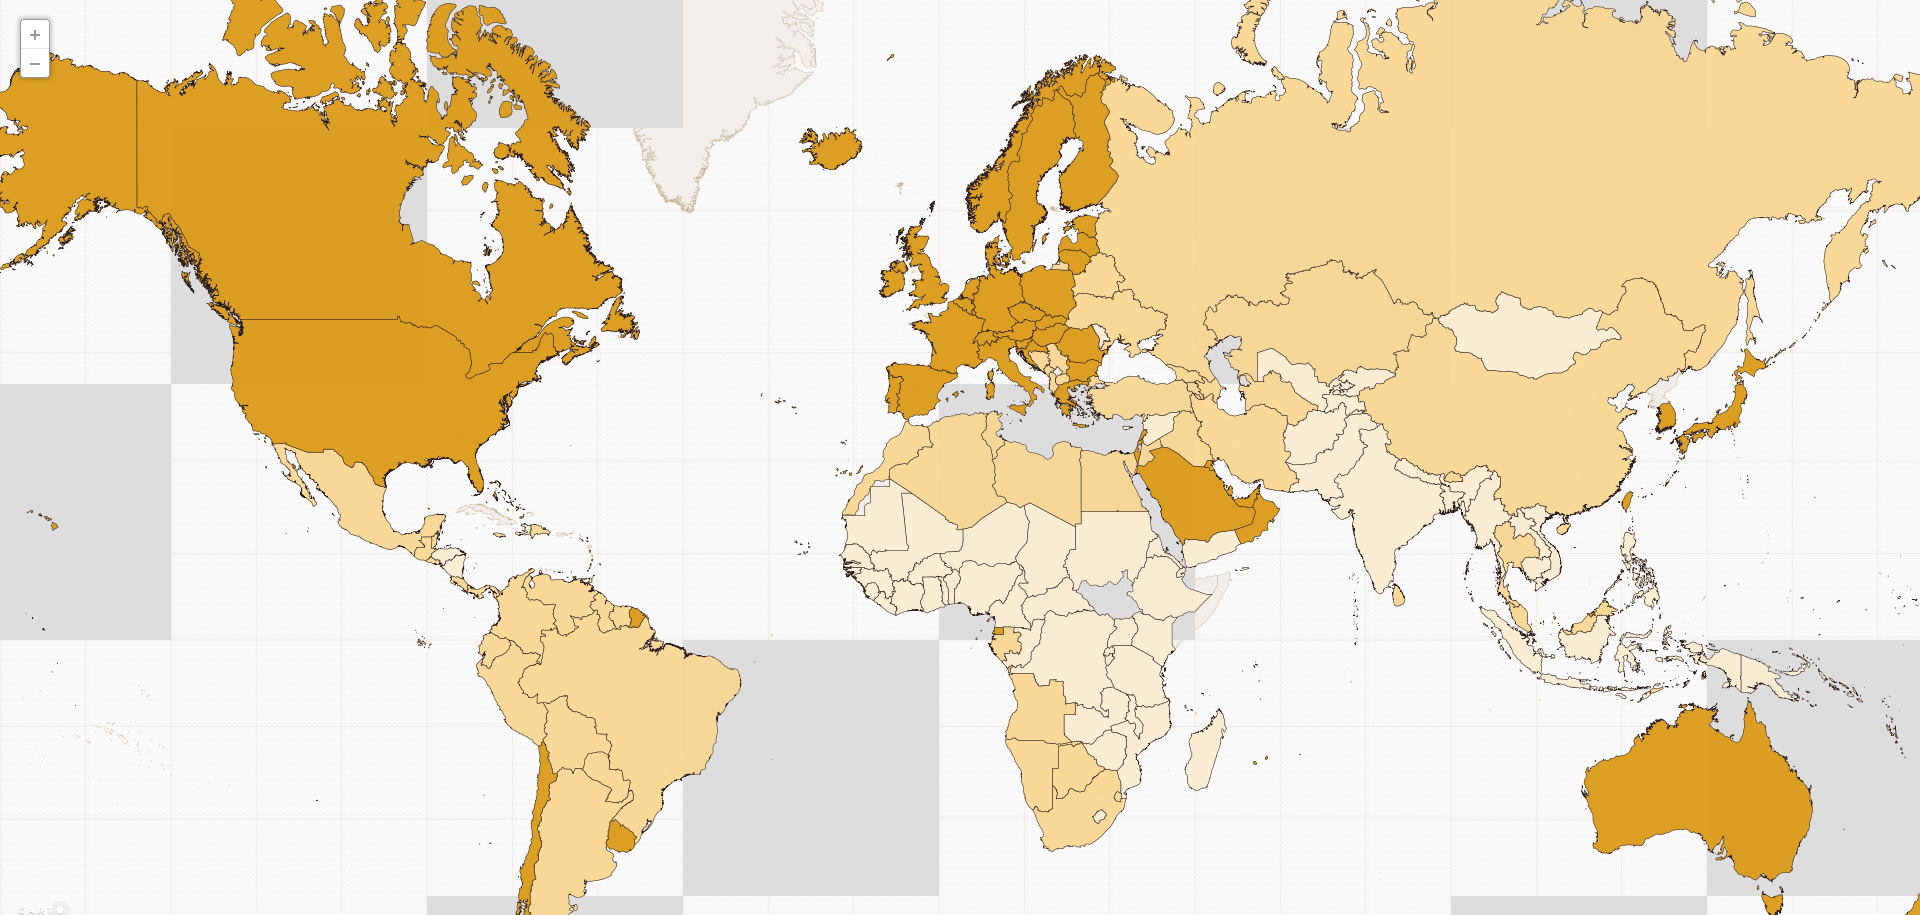
\includegraphics[scale=0.2]{ewaste_map.png}
\end{center}

\subsection{Normativa}
\subsubsection{Convenzione di Basilea}
Entrata in vigore dal 5 maggio 1992, ha come obiettivo la riduzione dei movimenti di rifiuti pericolosi (incluso anche il RAEE) da paesi sviluppati verso paesi in via di sviluppo. Prevede quindi:
\begin{itemize}
	\item \textbf{Divieto generale} su import ed export di rifiuti
	\item \textbf{Consenso}
	\item \textbf{Tracciabilità}
\end{itemize}
191 paesi l'hanno sottoscritta (188 delle UN, le isole Cook, la UE e la Palestina) ma non gli USA, il Timor Este, le isole Fiji, Haiti e il Sud Sudan.

\subsubsection{EU WEEE}
Nel 2018 è entrata in vigore la direttiva europea sull'e-waste, che ha come obiettivi:
\begin{itemize}
	\item Prevenire la \textbf{creazione} di e-waste
	\item Contribuire all'utilizzo intelligente delle risorse, oltre che al riuso, riciclo e recupero di materiali
	\item Migliorare l'impatto ambientale di tutti gli attori coinvolti nel ciclo di vita dei prodotti elettronici
\end{itemize}
Ogni anno in Unione Europea sono infatti prodotti 13.5 milioni di tonnellate di dispositivi elettronici, di cui 4.9 milioni diventano e-waste (circa 11Kg a persona).\\
La legge prevede:
\begin{itemize}
	\item Divisione e corretto smaltimento e riciclo dell'e-waste
	\item Combattere l'esportazione illegale di rifiuti tramite spedizioni camuffate
	\item Ridurre la burocrazia per l'unificazione dei registri dei dispositivi elettronici e i loro formati
\end{itemize}

\subsection{Obsolescenza programmata}
L'obsolescenza programmata è quando un prodotto è progettato per avere una durata più breve nel tempo.\\
Uno dei primi esempi è del 1925 quando aziende statunitensi ed europee produttrici di lampadine fondarono il \textbf{cartello Phoebus} che abbassò forzatamente l'aspettativa di vita delle lampadine da 2.500 ore a  1.000.\\
Ad oggi poi ci sono molteplici esempi, tra cui le cartucce delle stampanti, batterie non sostituibili, prese differenti (anche se dal 2024 in UE è illegale vendere dispositivi senza USB-C) e aggiornamenti programmati per rallentare i dispositivi.\\
Per implementare con successo l'obsolescenza programmata bisogna:
\begin{itemize}
	\item garantire che la durata di vita del prodotto sia sufficientemente lunga per sviluppare un \textbf{bisogno del cliente}
	\item il cliente deve ritenere che il prodotto sia di \textbf{qualità} anche se alla fine deve sostituirlo
\end{itemize}

\subsubsection{Obsolescenza percepita}
Quando un cliente è convinto di aver bisogno di un prodotto aggiornato anche se il quello già posseduto funziona bene. Ad esempio con le auto o i telefoni.

\subsection{Alimentazione delle infrastrutture digitali}
Nel 2009 Greenpeace fa il primo benchmark delle \textbf{prestazioni energetiche} del settore IT e sfida le maggiori aziende ad alimentare la loro crescita al $100\%$ con fonti rinnovabili. Nel 2013 Apple, Facebook e Google (seguite poi nel 2017 da altre 20 aziende del settore) assumono l'impegno di utilizzare al $100\%$ energie rinnovabili perché:
\begin{itemize}
	\item stava aumentando la \textbf{competitività} dei costi dell'energia rinnovabile
	\item iniziava ad esserci \textbf{preoccupazione} per il cambiamento climatico da parte di clienti e dipendenti
\end{itemize}
Dal 2010 l'acquisto di energia rinnovabile da parte delle aziende è aumentato drasticamente, arrivando a superare i $3,4GW$ nel 2015.

\subsubsection{Ostacoli}
I principali ostacoli all'adozione di fonti rinnovabili al $100\%$ sono:
\begin{itemize}
	\item Mancanza di \textbf{trasparenza} poiché le aziende sono riluttanti a pubblicare i dati energetici
	\item Mancanza di accesso alla fornitura di energia rinnovabile
\end{itemize}
\begin{center}
	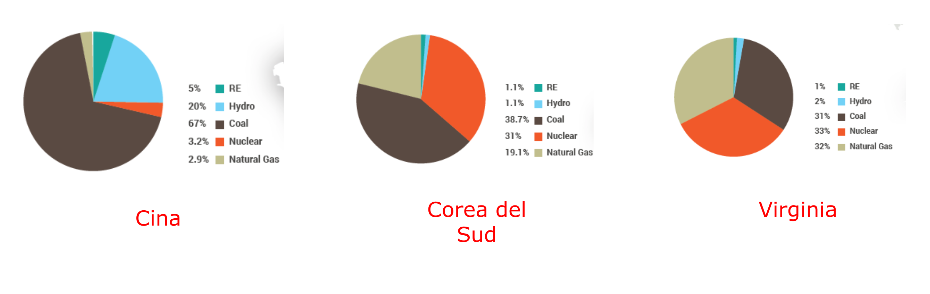
\includegraphics[scale=0.4]{energy_availability.png}
\end{center}

\subsubsection{Report}
L'ultimo report di Greenpeace (2017) si basa su dati che arrivano:
\begin{itemize}
	\item Direttamente dalle aziende
	\item Pubblicamente disponibili grazie a comunicazioni aziendali, comunicazioni pubbliche agli stakeholder, organismi di rendicontazione, copertura mediatica o rapporti pubblicati
\end{itemize}
I voti finali per ogni azienda sono determinati da:
\begin{itemize}
	\item \textbf{Trasparenza} al $20\%$
	\item \textbf{Impegno} per le energie rinnovabili e per le politiche di localizzazione al $20\%$
	\item \textbf{Efficienza energetica} e mitigazione dei gas serra al $10\%$
	\item Approvvigionamento di \textbf{energia rinnovabile} al $30\%$
	\item \textbf{Patrocinio} al $20\%$
\end{itemize}
Le conclusioni del report vedono Apple leader assieme a Google. Switch leader tra gli operatori di Cloud Computing. Amazon AWS in una zona grigia, in quanto non c'è sufficiente trasparenza e principalmente in crescita in luoghi principalmente serviti da energia non rinnovabile.
\begin{center}
	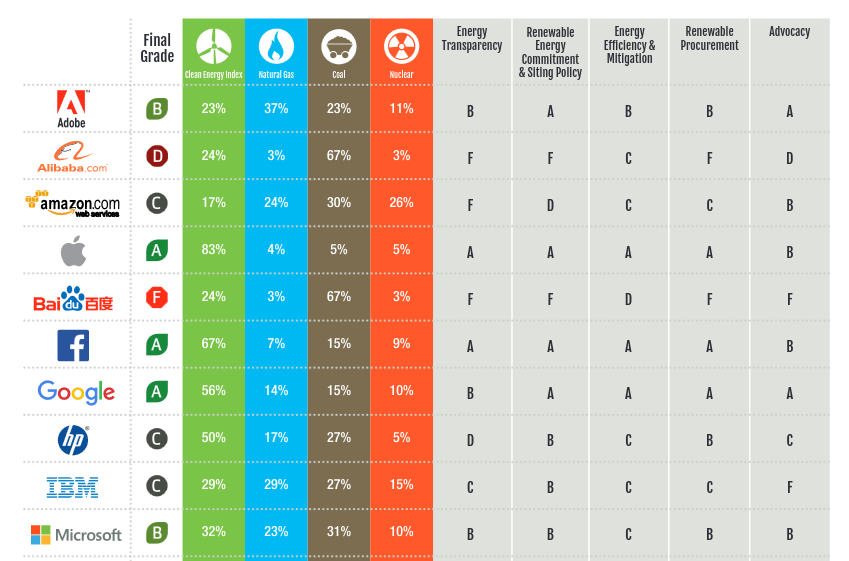
\includegraphics[scale=0.5]{greenpeace_report_1.png}
\end{center}
\begin{center}
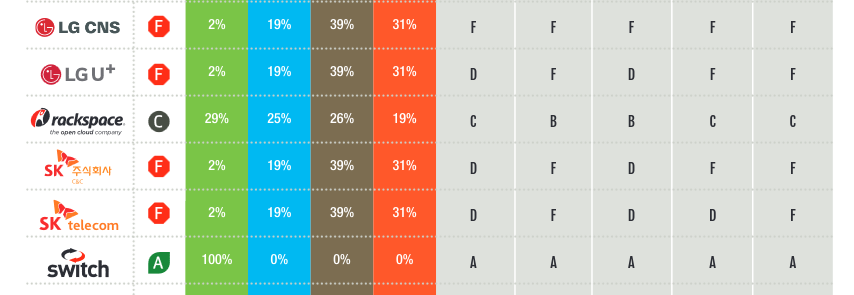
\includegraphics[scale=0.5]{greenpeace_report_2.png}
\end{center}
Ad oggi le aziende che erano leader nel 2017 continuano a spingere per l'uso delle energie rinnovabili e per il riciclo e il riuso (Google tra i tanti obiettivi ha lo $0\%$ di produzione di e-waste). Amazon continua ad essere in una zona grigia, facendo diverse buone azioni ma per la maggior parte non in ambito del cambiamento climatico. Facebook non ha pubblicato obiettivi ufficiali ma solamente il report annuale di sostenibilità.